%%%%%%%%%%%%%%%%%%%%%%%%%%%%%%%%%%%%%%%%%%%%%%%%%%%%%%%%%%%%%%
\section{Introdução}
\begin{frame}

    \frametitle{Histórico}

    \begin{itemize}
      \item Criada em 2013 por Neng-Fa Zhou e Jonathan Fruhman; 

      \item Utiliza o B-Prolog como base de implementação, e ambas utilizam 
      a Lógica de Primeira-Ordem (LPO) como seu fundamento;

      \item Uma evolução ao Prolog após seus mais de 40 anos de sucesso!

      \item Sua atual versão é a 2.5 (\today).

    \end{itemize}
\end{frame}

%%%%%%%%%%%%%%%%%%%%%%%%%%%%%%%%%%%%%%%%%%%%%%%%%%%%%%%%%%%%%%%%%%%%%

\subsection{Estrutura da Linguagem}

\begin{frame}
	\frametitle{Conhecendo PICAT}
    
    \begin{itemize}
    
    	\item Picat é uma linguagem que visa ser simples, mas ainda assim
        poderosa e multiuso;
        
        \item Por isso estão implementadas diversas características 
        normalmente não associadas com linguagens lógicas;
        
        \item Isto torna Picat uma linguagem essencialmente multiparadigma,
        abrangendo partes de ambos os paradigmas declarativo e imperativo;
        
        \item Esta combinação de características declarativas e imperativas permite
        o desenvolvimento de softwares mais produtivos, mas que ainda possam ser altamente 
        otimizados para tarefas específicas, ou softwares mais simples para tarefas mais mundanas;
        
    \end{itemize}
    
\end{frame}

%%%%%%%%%%%%%%%%%%%%%%%%%%%%%%%%%%%%%%%%%%%%%%%%%%%%%%%%%%%%%%%%%%%%%

\begin{frame}
    \frametitle{O que é ser Multiparadigma ?}

    \begin{itemize}
    
      \item Uma linguagem Multiparadigma é uma que contém características  de vários paradigmas de 
      programação.
      
      \item Picat abrange os seguintes paradigmas:
      
      \begin{itemize}
      	\item[--] Lógico
      	\item[--] Funcional
      	\item[--] Procedural
      \end{itemize}
      
      \item Uma boa \textit{mistura} de: Haskell (Funcional) , Prolog (Lógica) e 
      Python (Procedural e Funcional).
      
    \end{itemize}
      
      \begin{figure}
        \centering
        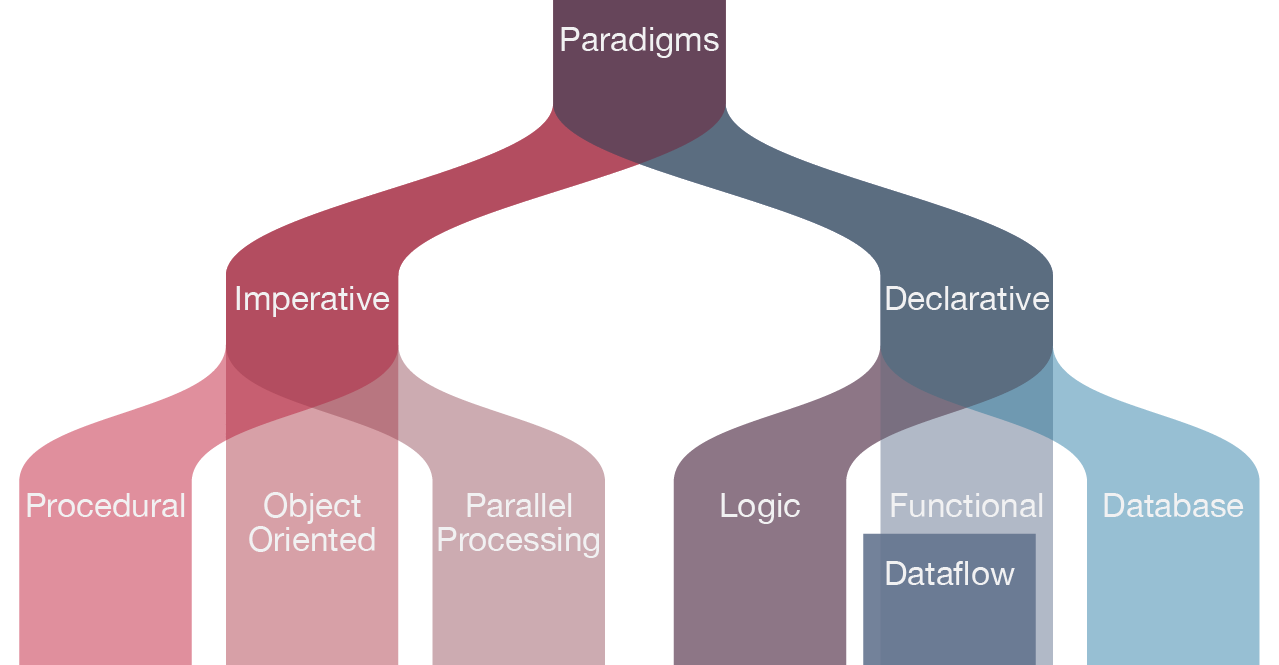
\includegraphics[width=.5\textwidth] {figures/Paradigma_Flow.png}
        \caption{Fluxograma dos paradigmas de programação.}
        \label{Fluxograma dos Paradigmas}
%       Fonte: http://www.danieldavis.com/wp-content/uploads/2013/09/paradigms.png
      \end{figure}
      

\end{frame}

%%%%%%%%%%%%%%%%%%%%%%%%%%%%%%%%%%%%%%%%%%%%%%%%%%%%%%%%%%%%%%%%%%%%%
\subsubsection{Paradigmas}
\begin{frame}
	\frametitle{Paradigma Lógico}
    
    \begin{itemize}
    
    	\item Uma linguagem lógica é uma onde o programa é expresso como uma série
        de predicados lógicos, usadas para expressar fatos e regras sobre um dado domínio;
    
    	\item Regras são escritas em formas de cláusulas, que são interpretadas como
        implicações lógicas;
        
        \item Este é o principal paradigma de Picat.
    \end{itemize}

\end{frame}

%%%%%%%%%%%%%%%%%%%%%%%%%%%%%%%%%%%%%%%%%%%%%%%%%%%%%%%%%%%%%%%%%%%%%

\begin{frame}
	\frametitle{Paradigma Funcional}
    
    \begin{itemize}
    
    	\item Uma linguagem funcional é uma onde os elementos do programa podem ser avaliados e 
        tratados como funções matemáticas;
        
         \item Um dos principais motivos de se usar linguagens funcionais é a previsibilidade
         e facilidade de entendimento do estado atual do programa;
         
         \item Isso anda lado a lado com a sintaxe simples e intuitiva de Picat, possibilitando
         que seja possível entender como um programa é estruturado e será executado com muita
         facilidade.
         
    \end{itemize}
    
    \begin{figure}
    	\vspace*{-3mm}
        \centering
        \caption{Comparação do paradigma funcional com outros paradigmas comuns}
        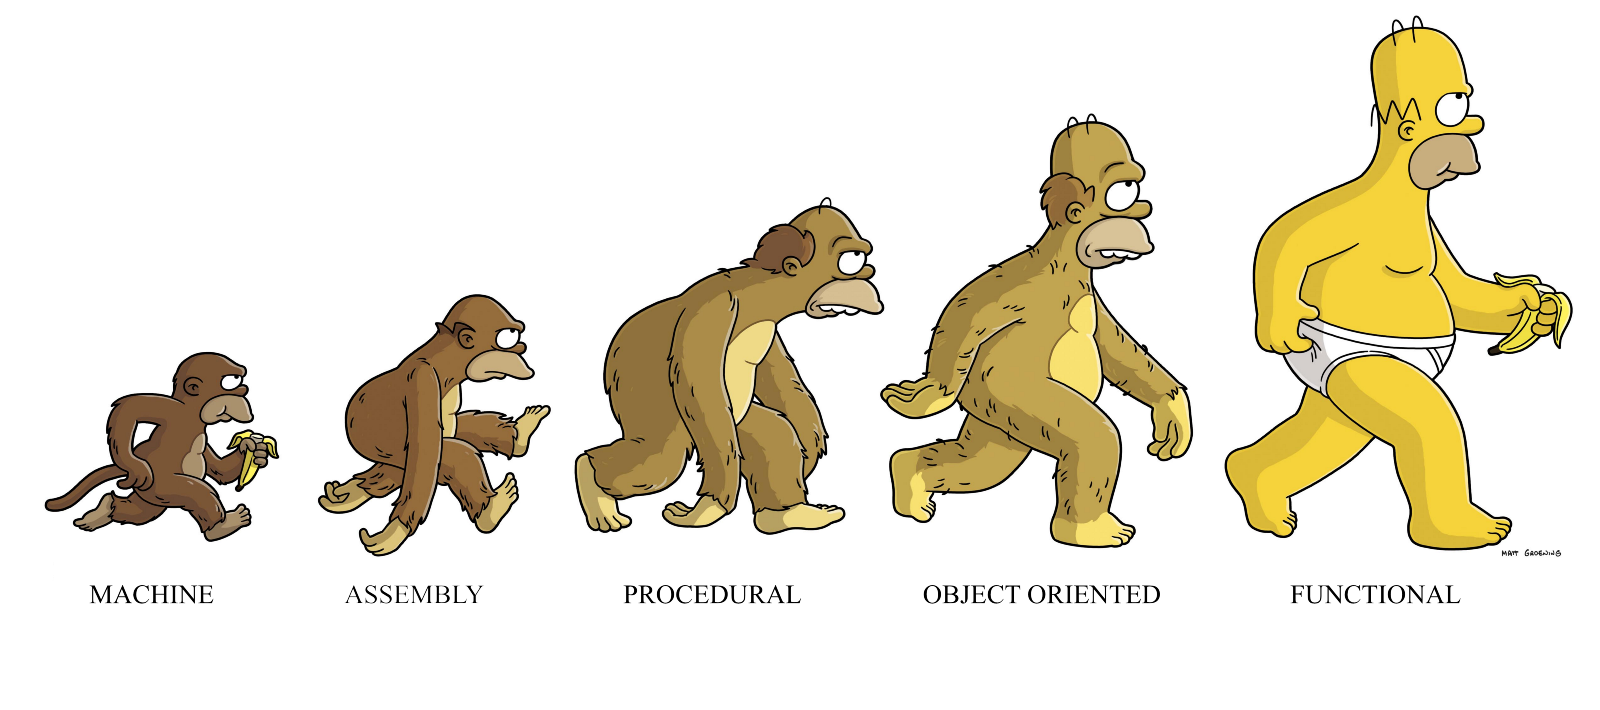
\includegraphics[width=.7\textwidth] {figures/Paradigma_Funcional.png}
        \label{Paradigma Funcional}
%       Fonte : https://medium.com/@cscalfani/so-you-want-to-be-a-functional-programmer-
% 		part-1-1f15e387e536
    \end{figure}
    
\end{frame}

%%%%%%%%%%%%%%%%%%%%%%%%%%%%%%%%%%%%%%%%%%%%%%%%%%%%%%%%%%%%%%%%%%%%%

\begin{frame}
	\frametitle{Paradigma Procedural}
    
    \begin{itemize}
    
    	\item Uma linguagem procedural é uma que pode ser subdividida em \textit{procedimentos},
        também chamados de rotinas, subrotinas ou funções;
        
        \item Em linguagens procedurais há um procedimento principal (geralmente chamado de 
        \textit{Main}) que controla o uso e a chamada de outros procedimentos, em Picat, o mesmo
        ocorre;
        
        \item Em Picat, cada premissa é tratada como um procedimento, que é resolvido por meio
        de métodos de inferência lógica;
       
    \end{itemize}
    
    \begin{figure}
    	\begin{columns}
    		\column{.6\linewidth}
	         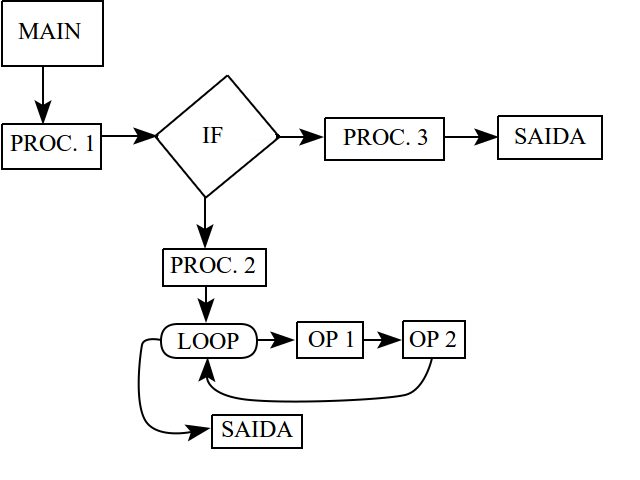
\includegraphics[width=.8\textwidth] {figures/Paradigma_Procedural.png}
             \column{.4\linewidth}
             \caption{Fluxograma representando a estrutura de um programa Procedural}
	         \label{Fluxograma Procedural}
		\end{columns}
	\end{figure}
    
\end{frame}

%%%%%%%%%%%%%%%%%%%%%%%%%%%%%%%%%%%%%%%%%%%%%%%%%%%%%%%%%%%%%%%%%%%%%

\begin{frame}
    \frametitle{Algumas Características:}

    \begin{itemize}
    
      \item Sintaxe elegante e simples, facilitando a leitura e entendimento do código;
      
      \item Alta velocidade de execução;
      
      \item Disponibilidade nos sistemas operacionais e arquiteturas mais importantes;
      
      \item \textit{Queries} $\Rightarrow$ Semelhante a Python, podem ser feitas \textit{queries}
      ou \textit{consultas} ao terminal de Picat, tais consultas podem ser qualquer tipo de 
      programa compilável pela linguagem, por menor que seja;
      % Melhorar essa descrição
      
      \item Várias bibliotecas da própria linguagem disponíveis, assim como diversas ferramentas
      externas possibilitam grande extensibilidade à linguagem.
      % Melhorar essa descrição
      
      
    \end{itemize}
\end{frame}

%%%%%%%%%%%%%%%%%%%%%%%%%%%%%%%%%%%%%%%%%%%%%%%%%%%%%%%%%%%%%%%%%%%%%

\subsection{Características}
\begin{frame}			  
    \frametitle{Acrônimo de \textbf{P.I.C.A.T.}}
  
  	\begin{description}
   
 
      \item [\textbf{P}:] \textit{Pattern-matching}:  Utiliza o conceito de \textit{casamento de 
      padrões}, equivalente aos conceitos de \textit{unificação} da LPO;

      \item [\textbf{I}:] \textit{Intuitive}: Oferece estruturas de decisão, atribuição e laços de
      repetição, etc. Análogo a outras linguagens de programação mais populares;

      \item [\textbf{C}:] \textit{Constraints}: Suporta a programação por restrições (PR) para 	
      problemas combinatórios;

       \item [\textbf{A}:] \textit{Actors}: Suporte as chamadas a eventos, os atores;

      \item [\textbf{T}:] \textit{Tabling}: Implementa a técnica de \textit{memoization}, com 
      soluções imediatas para problemas de Programação Dinâmica (PD).
   
  
  \end{description}	
\end{frame}

%%%%%%%%%%%%%%%%%%%%%%%%%%%%%%%%%%%%%%%%%%%%%%%%%%%%%%%%%%%%%%%%%%%%%

\subsubsection{Instalação}
\begin{frame}
    \frametitle{Instalação do PICAT}

  \begin{itemize}
  
  	\item Baixar a versão desejada de:\\ 
    \hspace{8mm} \url{http://picat-lang.org/download.html}
    
   	\item Descompactar. Em geral em: \textbf{/usr/local/Picat/}
    
    \item Criar um link simbólico (Linux) ou atalhos (Windows):\\ 
    
   	\hspace{8mm}\texttt{ln -s /usr/local/Picat/picat   \hspace{3mm}   /usr/bin/picat}
    
    \item Se quiser adicionar (opcional) uma variável de ambiente:\\
          \hspace{8mm} \texttt{PICATPATH=/usr/local/Picat/}\\
          \hspace{8mm} \texttt{export PICATPATH}

    \item Ou ainda, adicione o caminho: \texttt{PATH=\$PATH:/usr/local/Picat}

   	\item Finalmente, tenha um editor de texto apropriado.\\
    \hspace{8mm} Sugestão: \textit{Geany}, \textit{Sublime} ou \textit{Atom}.
     
    \item Se possível, escolha a sintaxe da linguagem \textit{Erlang}.
    
    
  \end{itemize}



\end{frame}

%%%%%%%%%%%%%%%%%%%%%%%%%%%%%%%%%%%%%%%%%%%%%%%%%%%%%%%%%%%%%%%%%%%%%

\subsubsection{Usando Picat}

\begin{frame}
  \frametitle{Usando Picat}
  	\begin{itemize}
    
      \item Picat é uma linguagem de multiplataforma, disponível em qualquer arquitetura de 
      processamento e também de sistema operacional;
      \item Os seus arquivos fontes utilizam a extensão \textbf{.pi}. Exemplo: \texttt{programa.pi}
      \item Há dois modos principais de utilização do Picat: 
      
      \begin{itemize}
      	\item[--] Modo interativo, onde seu código é digitado e compilado diretamente na linha de 
        comando;
      	\item[--] \textit{Modo console} onde o console só é utilizado para compilar seus programas.
      \end{itemize}
      
      \item Códigos executáveis 100\% \textbf{stand-alone}: ainda não!
      \item Neste quesito, estamos em igualdade com Java, Prolog e Python
     
    \end{itemize}
\end{frame}

%%%%%%%%%%%%%%%%%%%%%%%%%%%%%%%%%%%%%%%%%%%%%%%%%%%%%%%%%%%%%%%%%%%%%
